\paragraph{}

Podstawowymi aktywnościami projektu są moduły wyświetlania planet oraz obliczania pozycji planet. Jednak dla działania aplikacji bardzo ważne są również inne aktywności, które mimo, że prostsze w implementacji mają duży wpływ na architekturę projektu. Poniższy diagram przedstawia kolejne aktywności aplikacji podczas działania. Dodatkowo przedstawiony na diagramie jest przepływ najważniejszych informacji, czyli pozycji planet.

\paragraph{}

\begin{figure}[ht!]
	\centering
	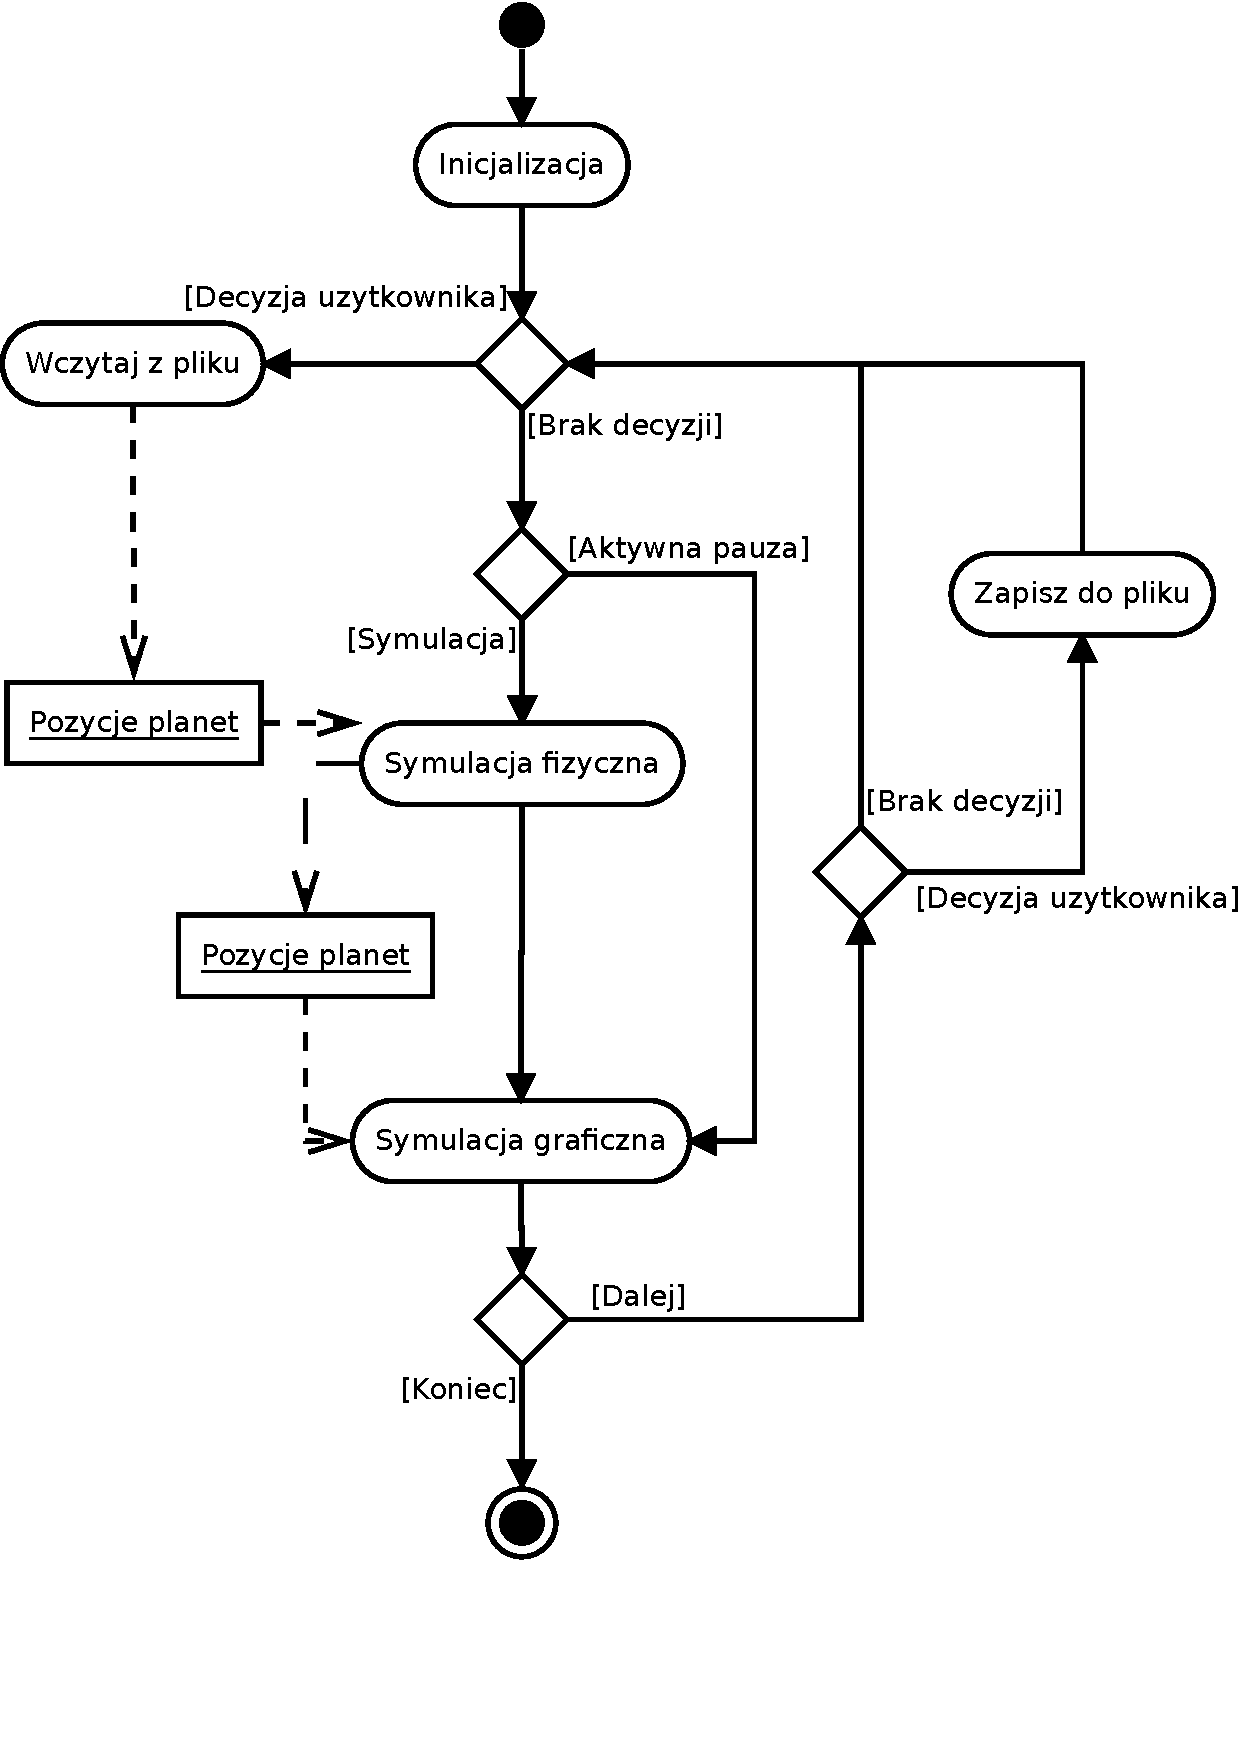
\includegraphics[width=0.75\textwidth]{activity.pdf}
	\caption{Diagram aktywności}
	\label{fig:activity}
\end{figure}


\begin{description}
	\item[Inicjalizacja aplikacji] \hfill \\
	Jest to pierwsza aktywność jaką wykonuje program. Składa się ona z inicjalizacji wszystkich modułów, w szczególności modułu graficznego i fizycznego. Zajmuje się także początkową alokacją pamięci i wczytaniem wszystkich potrzebnych zasobów, takich jak tekstury, modele oraz inne potrzebne dane.
	\item[Wczytanie z pliku] \hfill \\
	Jeśli użytkownik zdecyduje zacząć symulację z wcześniej przygotowanego pliku ta akcja jest za to odpowiedzialna. Musi ona załadować potrzebne dane z pliku oraz zapisać je poprzez pamięć RAM jednostki głównej do pamięci RAM jednostki graficznej. Użytkownik może również zdecydować o wczytaniu z pliku podczas już trwającej symulacji. W takim przypadku konieczne jest również zadbanie o odpowiednie wyczyszczenie poprzedniej symulacji, tak aby żadne artefakty nie zostały w pamięci RAM jednostki głównej ani graficznej.
	\item[Zapis do pliku] \hfill \\
	Na życzenie użytkownika aktualny stan symulacji może zostać zapisany do pliku. W takim przypadku zbierane z aplikacji są wszystkie potrzebne dane, takie jak pozycje planet, wielkości i ciężary planet, modele planet, pozycja kamery itp., oraz zapisywane są do pliku.
	\item[Aktywna pauza] \hfill \\
	Symulacja wspiera tak zwaną "aktywną pauzę". Oznacza to, że na żądanie użytkownika symulacja fizyczna jest zatrzymana, natomiast cały czas reszta aplikacji jest w pełni funkcjonalna. Oznacza to, że można sterować kamerą, wczytywać/zapisywać układy planetarne oraz dodawać/usuwać planety.
	\item[Symulacja fizyczna] \hfill \\
	Jest to kluczowy moduł dla działania aplikacji. Podczas każdej takiej aktywności obliczane są kolejne pozycje planet do wyświetlenia. W jednej takiej akcji może być obliczona więcej niż jedna klatka fizyczna, jeśli moc obliczeniowa komputera na to pozwala.
	\item[Symulacja graficzna] \hfill \\
	Ta aktywność odpowiedzialna jest przede wszytkim za wyświetlanie symulacji na ekranie. Głównym jej zadaniem jest wyświetlanie planet na ich pozycjach wraz z towarzyszącymi im efektami graficznymi. Pozycje planet do wyświetlenia pobierane są z modułu fizycznego. Jeśli natomiast jest włączona aktywna pauza i nowe pozycje nie zostały wygenerowane, moduł korzysta ze starych pozycji. Po zakończonej jednej iteracji pętli, aplikacja odczekuje chwilę, żeby nie zajmować całego procesora oraz żeby zapewnić takie samo działanie symulacji na słabszych komputerach (gdzie czekanie może zostać pominięte)
\end{description}

